\documentclass[12pt]{report}
\title{Enigma Machine}
\author{Eric Oliver}
\date{\today}

\setcounter{chapter}{5}

\usepackage{listings}
\usepackage{color}
\usepackage{graphicx}
\usepackage[margin=.5in]{geometry}

\definecolor{codegreen}{rgb}{0,0.6,0}
\definecolor{codegray}{rgb}{0.5,0.5,0.5}
\definecolor{codepurple}{rgb}{0.58,0,0.82}
\definecolor{backcolour}{rgb}{0.95,0.95,0.92}

\lstdefinestyle{mystyle}{
    backgroundcolor=\color{backcolour},   
    commentstyle=\color{codegreen},
    keywordstyle=\color{magenta},
    numberstyle=\tiny\color{codegray},
    stringstyle=\color{codepurple},
    basicstyle=\footnotesize,
    breakatwhitespace=false,         
    breaklines=true,                 
    captionpos=b,                    
    keepspaces=true,                 
    numbers=left,                    
    numbersep=5pt,                  
    showspaces=false,                
    showstringspaces=false,
    showtabs=false,                  
    tabsize=4
}

\lstset{style=mystyle}

\begin{document}
\maketitle

\lstinputlisting[language=python]{enigma.py}

\lstinputlisting[language=python]{enigma_net.py}

\begin{figure}[h]
    \centering
    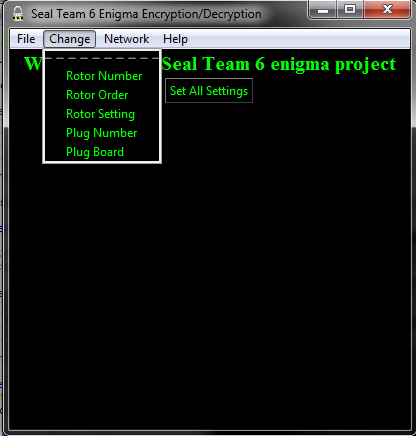
\includegraphics[scale=.5]{All_Settings.png}
    \caption{Settings for the GUI}
    \label{fig:settings}
\end{figure}

\begin{figure}[h]
    \centering
    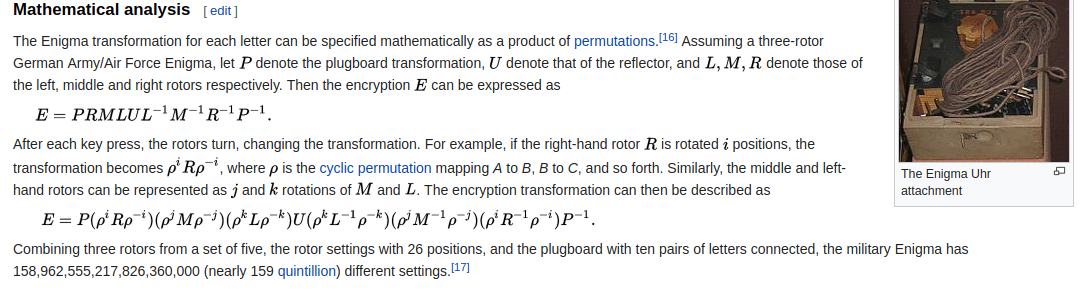
\includegraphics[scale=.5]{Complexity.png}
    \caption{Complexity Functions}
    \label{fig:complexity}
\end{figure}

\begin{figure}[h]
    \centering
    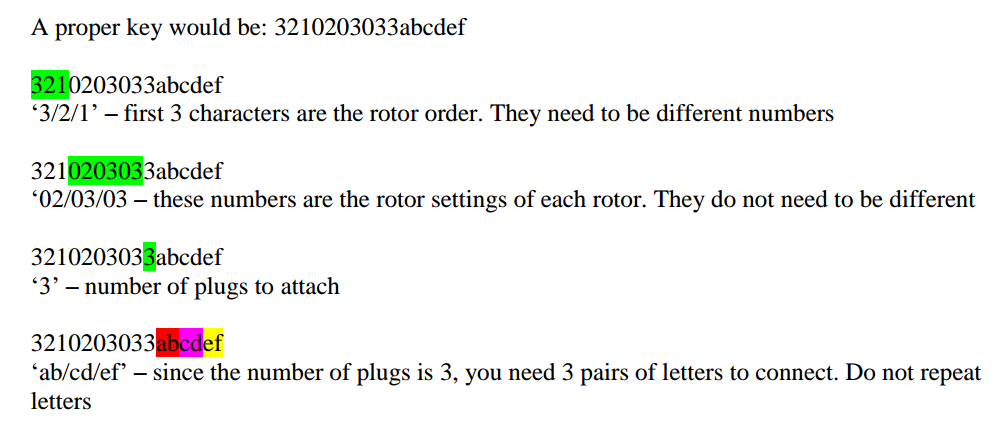
\includegraphics[scale=.5]{keyword.png}
    \caption{Keyword Structure}
    \label{fig:keyword}
\end{figure}

\begin{figure}[h]
    \centering
    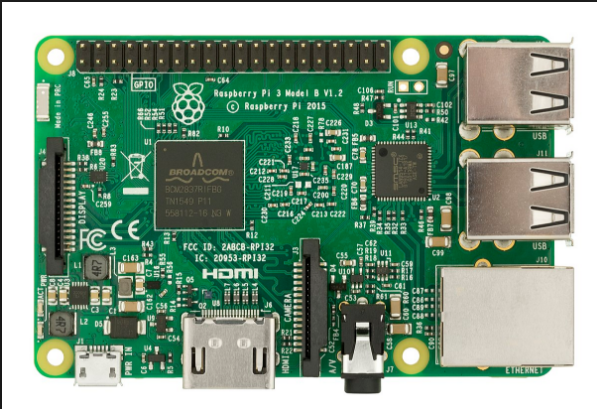
\includegraphics[scale=.5]{Raspberrypi.png}
    \caption{Raspberry Pi}
    \label{fig:rpi}
\end{figure}

\end{document}